%%%%%%%%%%%%%%%%%%%%%%%%%%%%%%%%%%%%%%%%%%%%%%
\section{Beam requirements}
\label{sec:beamrequirements}

The requested beam parameters are driven by the requirement that the results from the CERN test beam should be directly applicable to the future large underground single-phase LAr detector with minimal extrapolation. The CERN test beam data will be used to evaluate the detector performance, to understand the various physics systematic effects, and to provide data for event reconstruction studies that are representative of neutrino interactions. To satisfy the requirement, the beam parameters must span a broad range of particle momenta to match the charged particle spectrum and topologies that are expected in the DUNE far detector. The particle beam composition should consist of electrons, muons, and hadron and need to be charge-selected. The expected momentum distributions for secondary particles from neutrino interactions are shown in Figure~\ref{fig:particlemomenta}. There is a large spread in the momentum distribution with most particles peaked near 200 MeV/c.  
The desirable momentum range for ProtoDUNE-SP  is in the low momentum region. Based on the feedback and constraints from the CERN beam group, the requested beamline design allows the transport of beam particles from about 0.5 GeV/c up to 7 GeV/c. 

\fixme{here a part that cam stay here or in the run plan section..or
  nowhere..}
Preliminary beam simulations show that the hadron rates at 
energies below 1~GeV/c are low. Moreover, low energy beams are more
subject to disruption and degradation by materials in the
beamline. Therefore, the beam program factors in the beam composition and also takes
into account of particle interaction topologies.  Full FLUKA\cite{fluka05,Fluka15}
 simulations
of particle transport in the the ProtoDUNE detector, including the
beam window, have been performed.
 The physics requirement is the possibility to measure
 stopping particles and  interactions both at high and at low energies.    
%For stopping, the “initial “energy has small meaning
At 1 GeV/c, still 35\% of protons do stop, while they reduce to only 5
per mill at 2 GeV/c.  At  1 GeV/c  the protons interact at all
energies as shown in
Figure~\ref{fig:pandpiint}. The residual energy at the interaction
point can be reconstructed by measuring the energy deposit along the proton track.
Many of the  low energy pions decay in the 37~m between the secondary target
and the LAr volume.  The fraction of stopping $\pi$ for one $\pi$
leaving the target is 3\% at P=0.4~GeV/c still  1.3\% at P=0.7~GeV/c,
then decreases.  Having a $\pi$ beam at 0.7~GeV/c still allows to
measure pion interactions down to few tens of MeV with good
statistics. In a 1~GeV/c beam, the low energy interactions are still
present albeit with lower rate, as shown in Figure~\ref{fig:pandpiint}.
%\fixme{also need to address particle interaction topologies}
For what concerns Kaons, the length of the beam line is such that no
$K$ arrives at the detector for momenta lower than $\approx$2~GeV/c.
For what concerns electrons, the peculiar topology of very low energy
showers requires to measure at the lowest possible momenta.
\begin{cdrfigure}[Energy at interaction]{pandpiint}{Kinetic energy of
    particles at the point of interaction in the ProtoDUNE active
    volume, for different beam momenta. Histograms are normalized to one particle injected in the
    beamline acceptance. FLUKA simulations include the beam window
    materials, beam are considered as monochromatic and
    parallel. left: protons, right: pions.}
  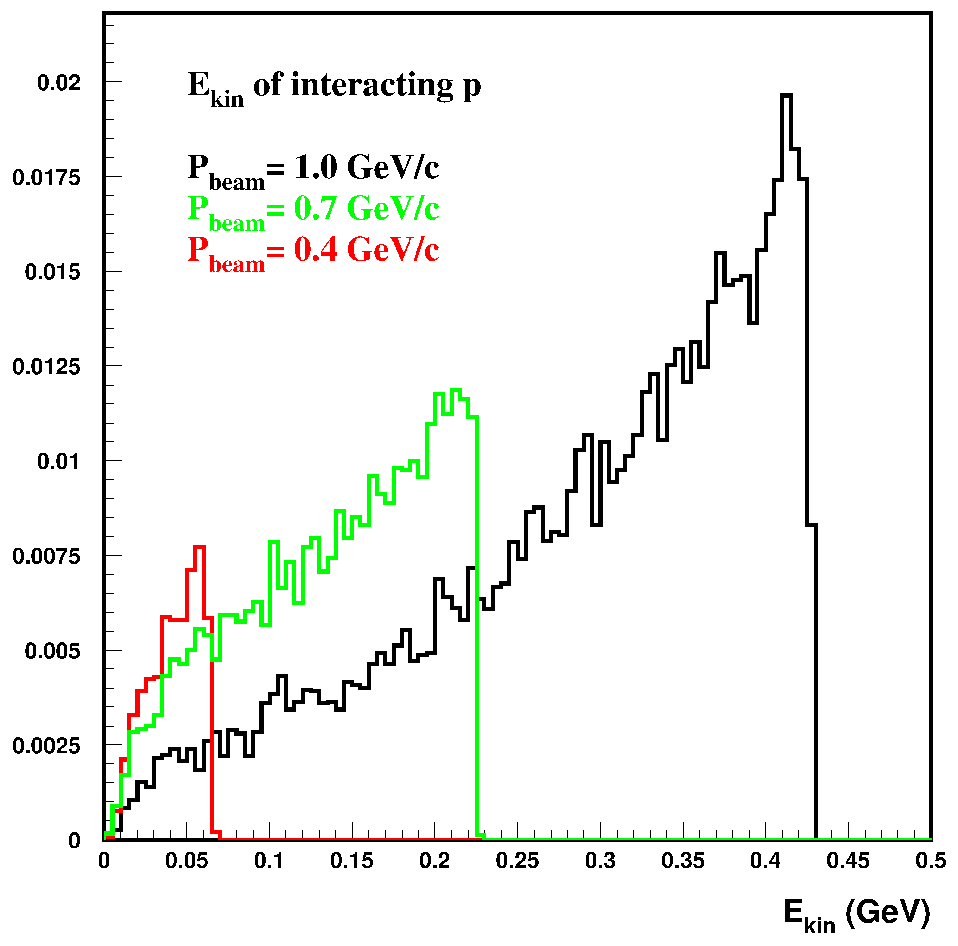
\includegraphics[width=0.49\textwidth]{pvarie_intene.pdf}
  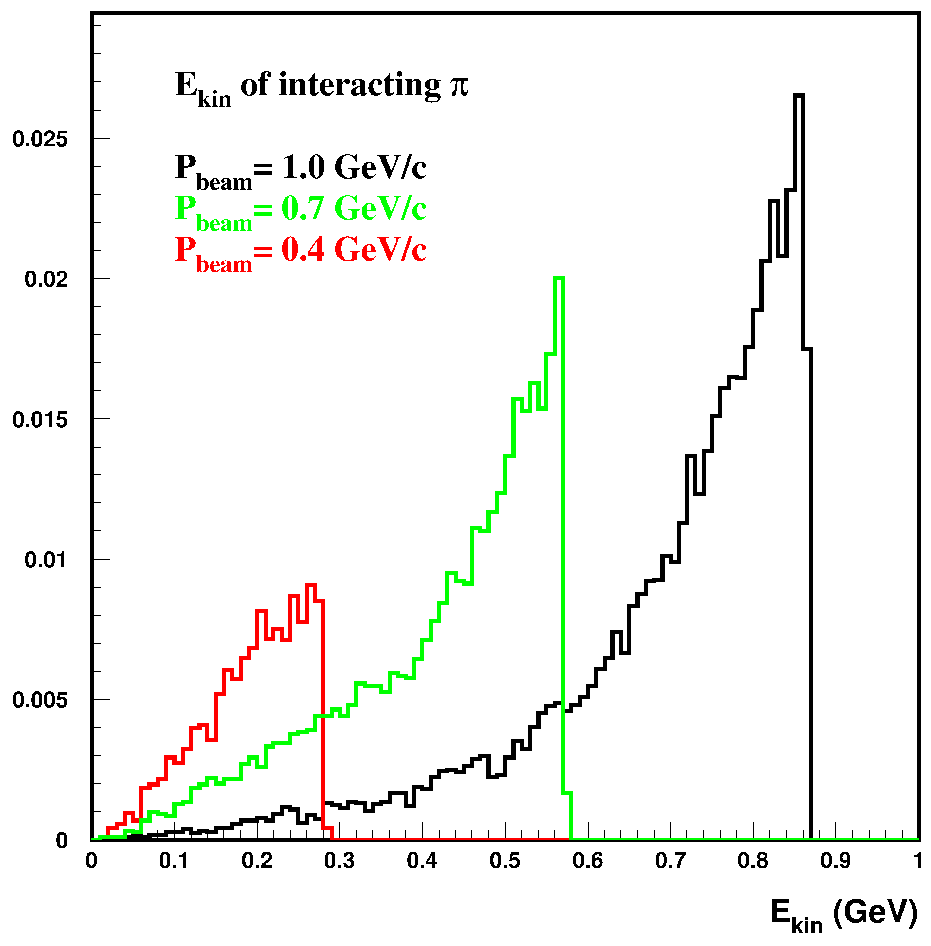
\includegraphics[width=0.49\textwidth]{pivarie_intene.pdf}
\end{cdrfigure}
%% end of   part that can go either here or in the run plan 


The maximum electron drift time in the TPC is about 2.25 ms. In order
to keep the  pile-up in the TPC at the percent-level, the planned
beam rate should be about 100 Hz.  
The ProtoDUNE-SP TPC has two drift volumes separated by a
passive cathode plane. It is desirable to aim the particle beam such
that a large fraction of the lower energy hadronic showers are mostly
contained in one drift volume, thus minimizing the uncertainties from
particles lost in the inactive detector materials. It is also
important to be able to inject beam into the cryostat at multiple
locations to study the detector
response. Figure~\ref{fig:beamwindow_loc} shows the three proposed
beam injection points.  The angles of the beam, w.r.t. the APA plane
are 3$^\circ$ (beam \#1), 8$^\circ$ (beam \#2), and 12$^\circ$ (beam
\#3). Due to engineering and safety considerations, only beam \#3 will
be fully instrumented with the beam window system as described in
Sections~\ref{subsec:beamwindow} and~\ref{sec:beamplug}. The remaining two beam positions will have
partial installation of the beam window system. With this
configuration, beam \#3 is the primary beam where most of the physics
data will be taken.
\begin{cdrfigure}[Beam window locations]{beamwindow_loc}{Planned beam window locations.}
  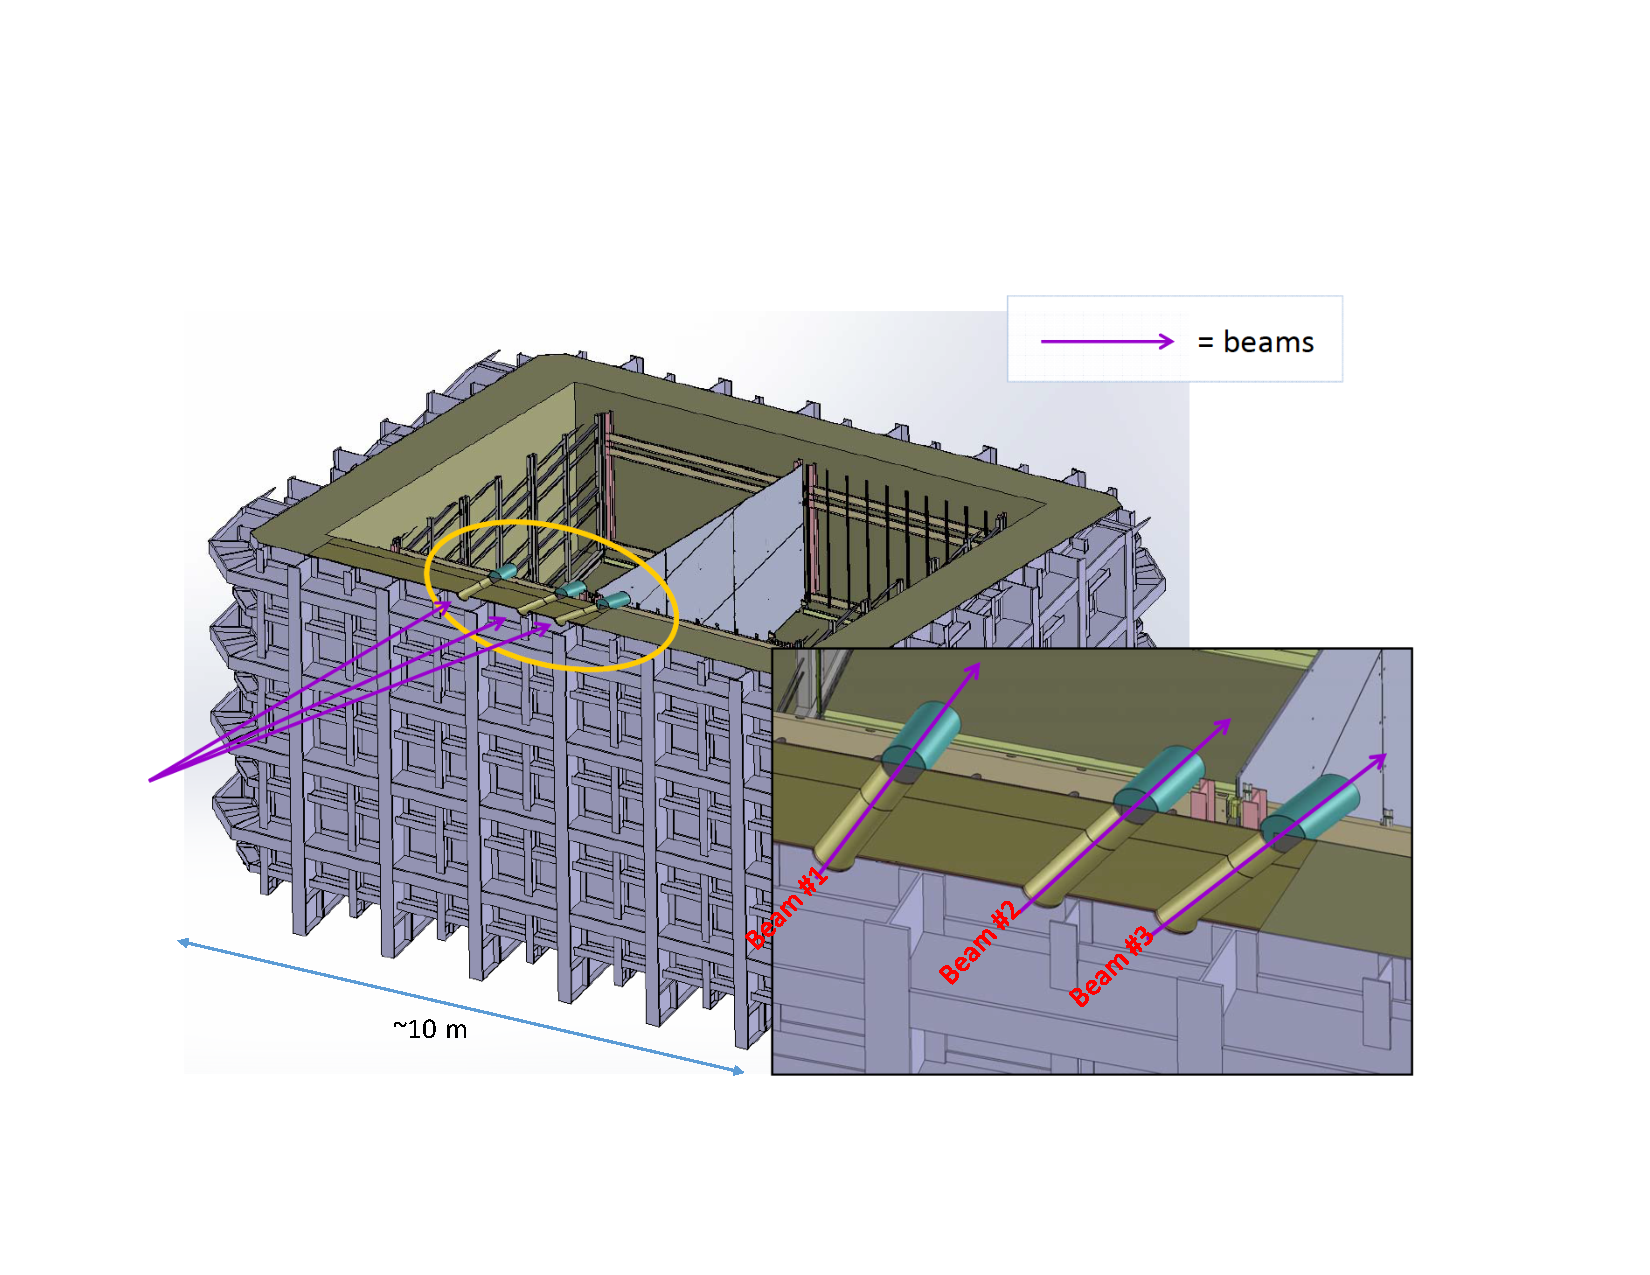
\includegraphics[width=0.9\textwidth]{beamwindow_locations.pdf}
\end{cdrfigure}
The summary of the beam requirements are shown in Table~\ref{tab:beamspecs}.
\begin{cdrtable}[Particle beam requirement]{cc}{beamspecs}{Particle beam requirements. (No Kaon is expected for beam momentum below 1 GeV/c.)}
%\textbf{Parameter } & \textbf{Requirements}  \\ \hline
 Parameter & Requirements \\ \toprowrule
  Particle Types        & $e^\pm,\mu^\pm,\pi^\pm$,$(K)$,$p$  \\ \colhline
  Momentum Range   & 0.5 - 7 GeV/$c$ \\ \colhline
  Momentum Spread   & $\Delta p/p  < $5 \% \\
  & (limited by the aperture of the magnets)  \\ \colhline
  Transverse Beam Size   & RMS(x,y) $\approx$ 1 cm  \\
  & (At the entrance face of the LAr cryostat) \\ \colhline
  Beam Divergence & tbd   \\ \colhline
  Beam Entrance Position & Multiple beam windows    \\ \colhline
  Rates & 100 Hz (maximum)    \\ \colhline
\end{cdrtable}
\fixme{ this table is a mix of requirements and properties  (i.e. the momentum spread is not a requirement, the beam size comes from optics, what about divergency?) maybe should be limited to real requirements}  
\fixme{put K in parentheses and provide appropriate moment in caption; lower momentum range should be 0.5 GeV (see CERN workshop discussion) }
\fixme{momentum spread/characterization: need tomato clear that this is w/o any beam monitor information}
\fixme{we should have beam divergence estimates from H2 and H4 simulation files}
\fixme{rate: max of 100 Hx; nominal 25Hz with goal to achieve 50 Hz (see CERN workshop)}
